\section{Illustrative examples}\label{sec:tutorials}

After installing preCICE, a user typically wants to run a first coupled example case as close to their application and preferred solvers as possible. Such an example needs to be simple enough to follow without significant expertise in any of the involved solvers, but yet full-featured in terms of coupling. With this in mind, we offer a collection of tutorial cases hosted on \github{precice/tutorials}, with step-by-step guides in the preCICE documentation\footnote{preCICE tutorials documentation: \url{https://precice.org/tutorials.html}}. Such a tutorial consists of all the required instructions and configuration files necessary to run the coupled simulation, as well as convenience scripts to run, visualize, and cleanup each case. The same cases and scripts are also used in the preCICE system tests (cf.~\autoref{ssec:system_tests}) and all tutorials follow a consistent structure and naming scheme, described in the contributing guidelines\footnote{preCICE contributing guidelines: \url{https://precice.org/community-contribute-to-precice.html}}.

An important design decision of these tutorials is that every combination of the available solvers should work and give reasonably similar results,
demonstrating the plug-and-play concept of preCICE. This lets the user start from a case as close to their target as possible
and then potentially replace one of the participants with their own solver, maintaining a reference to compare with.
To achieve this goal, we had to develop features that may otherwise seem unnatural.
One of the most prominent such features is that the adapters for OpenFOAM and CalculiX (natively 3D solvers) can also work
in a \emph{2D mode}, coupling only lines of face points instead of surfaces. This automatic 2D mode works either by applying
additional interpolation to map points from the mesh nodes to the face centers, or directly switching to data available at the face centers
or to data on a predefined plane. Even if the domain in that case appears to have an out-of-plane thickness, this is only there
for the solver configuration and not important for the coupling.

Historically, the collection has grown with contributions from the community. As such, the tutorials should currently be seen as individual examples showcasing particular applications and features, rather than as a structured cookbook. We focus here on two representative cases that are available for a wide range of solvers: a CHT and an FSI example. The complete collection of tutorials is listed in~\autoref{fig:tutorials-list}.

\begin{figure}[h!]
\centering
\small
\begin{framed}
\begin{minipage}{\textwidth}
  \begin{minipage}{0.5\textwidth}
    \begin{itemize}[leftmargin=*]
      \item \textbf{Quickstart:} A 2D case coupling a channel flow in OpenFOAM with an in-house rigid body motion solver in C++.
      This is meant as the single first tutorial a new user should try, requiring as few components as possible.
      \item \textbf{Flow in a channel with a perpendicular flap:} A 2D FSI tutorial with OpenFOAM, SU2, deal.II, FEniCS, Nutils, and CalculiX.
      \item \textbf{Flow over a heated plate:} A 2D CHT tutorial with OpenFOAM, FEniCS, and Nutils.
      \item \textbf{Partitioned heat conduction:} A 2D heat conduction tutorial with FEniCS, Nutils, and OpenFOAM.
      \item \textbf{Turek-Hron FSI3:} An FSI tutorial based on the benchmark described at~\cite{turek2006proposal}, with OpenFOAM and deal.II.
      \item \textbf{Multiple perpendicular flaps:} A three-field FSI tutorial (fully implicit coupling, transient) with OpenFOAM and deal.II.
      \item \textbf{3D elastic tube:} A 3D FSI tutorial with OpenFOAM and CalculiX.
    \end{itemize}  
  \end{minipage}\hfill
  \begin{minipage}{0.5\textwidth}
    \begin{itemize}
      \item \textbf{1D elastic tube:} A 1D FSI tutorial with toy solvers in Python and C++.
      \item \textbf{Flow over a heated plate -- nearest projection:} A nearest-projection mapping variant of the \emph{flow over a heated plate} tutorial, with OpenFOAM.
      \item \textbf{Flow over a heated plate -- steady state:} A steady-state variant of the \emph{flow over a heated plate} tutorial, with OpenFOAM and code\_aster.
      \item \textbf{Heat exchanger:} A three-field CHT tutorial (explicit coupling, steady state) with OpenFOAM and CalculiX.
      \item \textbf{Partitioned heat conduction -- complex setup:} A variant of the \emph{partitioned heat conduction} tutorial with a more complex geometry, with FEniCS.
      \item \textbf{Partitioned beam:} A structure-structure coupling tutorial with CalculiX.
      \item \textbf{Partitioned pipe:} A fluid-fluid coupling tutorial with OpenFOAM.
    \end{itemize}
  \end{minipage}
\end{minipage}
\end{framed}
\caption{List of available tutorial cases}
\label{fig:tutorials-list}
\end{figure}

\subsection{Flow over a heated plate CHT tutorial}

This tutorial consists of a simple CHT scenario with a relatively low runtime. Since experimental data is available by Vynnycky et al.~\cite{vynnycky1998forced} the scenario serves often as a validation case for CHT simulations (\cite{Birken2010, birken2015fast}). The case consists of a 2D channel flow, coupled at its bottom with a 2D heated solid plate (cf.~\autoref{fig:cht_setup}).
As heat is conducted across the solid plate, the temperature of the flow region above and downstream the plate increases, as shown in~\autoref{fig:cht_temperature}. We discuss here the transient variant of this tutorial\footnote{Documentation of this CHT tutorial: \url{https://precice.org/tutorials-flow-over-heated-plate.html}}. 
%In addition, two alternative tutorial variants are available: a steady-state case and a case demonstrating configuration changes for nearest-projection mapping.

\begin{figure}[h!]
\begin{center}
\strut\vspace*{-\baselineskip}\newline
\input{figs/plate/tikzcode.tex}
\end{center}

\begin{minipage}[t]{\textwidth}
\begin{minipage}[t]{.2\textwidth}
\begin{footnotesize}
\begin{center}
\begin{tabular}[t]{c S[table-format=1.2] s}
\multicolumn{3}{c}{Dimensions}\\
\midrule
$L$ & 3.50 & \meter\\
$H$ & 0.50 & \meter\\
$l$ & 0.50 & \meter\\
$h$ & 0.25 & \meter\\
$w$ & 1.00 & \meter\\
$z$ & 0.40 & \meter
\end{tabular}
\end{center}
\end{footnotesize}
\end{minipage}
\begin{minipage}[t]{.4\textwidth}
\begin{footnotesize}
\begin{center}
\begin{tabular}[t]{c S[table-format=4.3e2] s}
\multicolumn{3}{c}{Fluid}\\
\midrule
$u_\text{inflow}$ & 1e-1 & \meter\per\second\\
$T_\text{inflow}$ & 3e2  & \kelvin\\
$p_0$ & 1.035e5 & \pascal\\
$g$        & 9.81 & \meter\per\second\squared\\  % gravitational acceleration, https://github.com/precice/openfoam-adapter/blob/8ae5f061ab26ae059b8cdcf304089306f9ce7227/tutorials/CHT/flow-over-plate/buoyantPimpleFoam-laplacianFoam/Fluid/constant/g#L19
$k_F$      & 1e2  & \watt\per\meter\per\kelvin\\ % (follows from \frac{c_p \mu}{\text{Pr}}=k) 
$c_{p,F}$  & 5e3  & \joule\per\kilogram\per\kelvin\\  % specific heat capacity https://en.wikipedia.org/wiki/Specific_heat_capacity, https://github.com/precice/openfoam-adapter/blob/8ae5f061ab26ae059b8cdcf304089306f9ce7227/tutorials/CHT/flow-over-plate/buoyantPimpleFoam-laplacianFoam/Fluid/constant/thermophysicalProperties#L38
$\mu$      & 2e-4 & \kilogram\per\meter\per\second\\  % dynamic viscosity, https://github.com/precice/openfoam-adapter/blob/8ae5f061ab26ae059b8cdcf304089306f9ce7227/tutorials/CHT/flow-over-plate/buoyantPimpleFoam-laplacianFoam/Fluid/constant/thermophysicalProperties#L43
$\rho_F$   & 1  & \kilogram\per\meter\cubed \\ % https://github.com/precice/tutorials/issues/226
$\nu^*$ & 2e-4 & \meter\squared\per\second\\
$\text{Pr}^*$& 1e-2 & \\  % Prandtl number, https://en.wikipedia.org/wiki/Prandtl_number, https://github.com/precice/openfoam-adapter/blob/8ae5f061ab26ae059b8cdcf304089306f9ce7227/tutorials/CHT/flow-over-plate/buoyantPimpleFoam-laplacianFoam/Fluid/constant/thermophysicalProperties#L44
$\text{M}^*$& 24.10 & \kilogram\per\mol \\  % Molar mass https://github.com/precice/tutorials/blob/6d90ae3eb179113beb400e472c8832e29a48db9b/flow-over-heated-plate/fluid-openfoam/constant/thermophysicalProperties#L34
\end{tabular}
\end{center}
\end{footnotesize}
\end{minipage}
\begin{minipage}[t]{.4\textwidth}
\begin{footnotesize}
\begin{center}
\begin{tabular}[t]{c S[table-format=4.3e2] s}
\multicolumn{3}{c}{Solid}\\
\midrule
$T_\text{hot}$ & 3.1e2 & \kelvin\\
$k_S$          & 1e2   & \watt\per\meter\per\kelvin \\  % thermal conductivity, FEniCS: https://github.com/precice/tutorials/blob/5f4031fc7e45807dca787a525569b39a1909d2a3/CHT/flow-over-plate/buoyantPimpleFoam-fenics/Solid/heat.py#L100, OF: https://github.com/precice/openfoam-adapter/blob/8ae5f061ab26ae059b8cdcf304089306f9ce7227/tutorials/CHT/flow-over-plate/buoyantPimpleFoam-laplacianFoam/Solid/system/preciceDict#L37
$c_{p,F}$        & 1e2 & \joule\per\kilogram\per\kelvin\\
$\rho_S$         & 1 & \kilogram\per\meter\cubed \\  % https://github.com/precice/tutorials/issues/226
$\alpha_S^*$       & 1     & \meter\squared\per\second\\  % thermal diffusivity, FEniCS: https://github.com/precice/tutorials/blob/5f4031fc7e45807dca787a525569b39a1909d2a3/CHT/flow-over-plate/buoyantPimpleFoam-fenics/Solid/heat.py#L99, OF: https://github.com/precice/openfoam-adapter/blob/8ae5f061ab26ae059b8cdcf304089306f9ce7227/tutorials/CHT/flow-over-plate/buoyantPimpleFoam-laplacianFoam/Solid/constant/transportProperties#L18
\end{tabular}
\end{center}
\end{footnotesize}
\end{minipage}
\end{minipage}

\caption{Flow over a heated plate CHT tutorial: The setup is depicted at the top, geometric and physical parameters are listed in the tables at the bottom of the figure. The fluid participant reads heat flux at the interface $\Gamma_C$, while the solid participant reads temperature. The boundary values for the inflow ($\Gamma_\text{inflow}$), outflow ($\Gamma_\text{outflow}$), and the hot bottom of the plate ($\Gamma_\text{hot}$) are listed in the tables at the bottom of the figure. All other boundaries are insulated. $u_\text{inflow}$, $T_\text{inflow}$: velocity and temperature at the inflow boundary. $p_0$: ambient pressure at all boundaries of the fluid. $T_\text{hot}$: temperature at the bottom of the plate. $g$: acceleration due to gravity. $k_F$ and $k_S$: thermal conductivity of the fluid and solid. $\rho_F$ and $\rho_S$: density of the fluid and solid. $c_{p,F}$ and $c_{p,S}$: specific heat capacity of the fluid and solid. $\alpha_S^* = k_S / (\rho_S c_{p,S})$: thermal diffusivity of the solid. $\mu$: dynamic viscosity. $\nu^* = \mu / \rho_F$: kinematic viscosity. $\text{Pr}^* = c_{p,F} \mu / k_F$: Prandtl number of the fluid. $M^* = \rho_F R T_\text{inflow} / p_0$: Molar mass of the fluid with $R$ being the gas constant. $z$ is the out-of-plane thickness: even if the coupled case is described as 2D, OpenFOAM is still a 3D solver. Quantities marked with a $^*$ are derived quantities.}
\label{fig:cht_setup}
\end{figure}

\begin{figure}[h!]
\begin{center}
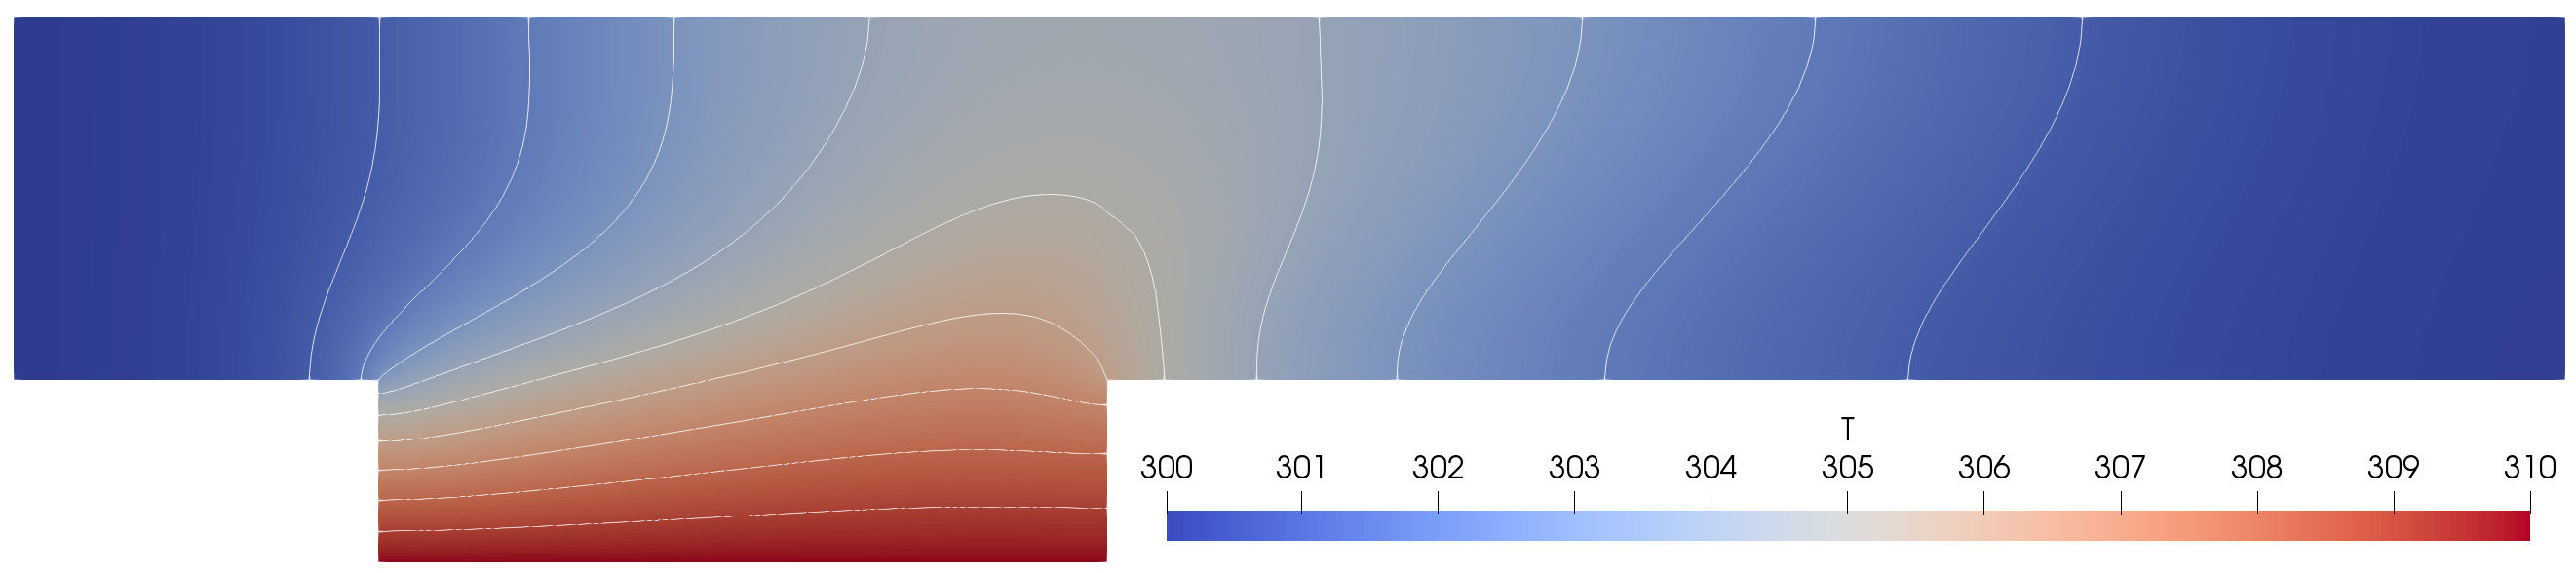
\includegraphics[width=\textwidth]{figs/plate-paraview/paraview10s.png}
\end{center}
\caption{Flow over a heated plate CHT tutorial: Isothermal lines for the OpenFOAM-FEniCS combination at time $t=10s$. The lines are continuous and smooth across the interface. Similar results are observed for all other solver combinations.}
\label{fig:cht_temperature}
\end{figure}

The fluid participant is the compressible OpenFOAM solver buoyantPimpleFoam.
% The fluid mesh consists of $293 \times 41 \times 1$ hexahedral cells and is denser per $x$ around the interface. As OpenFOAM is a 3D solver, we have to define a channel thickness (here $\SI{0.4}{\meter}$), but we only couple the line of cell centers at the interface. We also have to input a Prandtl number, which in this case we set to $\text{Pr} = \frac{c_p \mu}{k_F} = 0.01$.
For the solid participant, the user can choose among the OpenFOAM solver laplacianFoam and heat conduction solver examples based on FEniCS or Nutils.
In the case of laplacianFoam, we compute the heat flux assuming a constant heat conductivity $k_S$, which is additionally specified in the OpenFOAM adapter. In the case of FEniCS, the solver was developed as part of~\cite{QNWI} based on a heat equation example from~\cite{Langtangen2016}. A detailed description of the solver can be found in~\cite{rodenberg2021fenicsprecice}. In case of Nutils, we provide a similar example.

All of the possible combinations ($\{\text{OpenFOAM}\} \times \{\text{OpenFOAM, FEniCS, Nutils}\}$) use the same preCICE configuration file
and the user can select any combination at runtime. The solid participant solvers write heat flux values and apply a Dirichlet boundary condition by reading temperature values at the coupling interface. Accordingly, the fluid OpenFOAM participant writes temperature values and applies a Neumann boundary condition by reading heat flux values at the coupling interface. By default, the tutorial is configured with a serial-implicit coupling scheme in combination with Aitken under-relaxation and nearest-neighbor mappings.

A quantity that is commonly monitored in this scenario is the non-dimensional temperature $\theta = (T-T_\infty)/(T_h-T_\infty)$
along the interface. \autoref{fig:cht_results} depicts identical $\theta$ profiles for all solver combinations. Furthermore, the isothermal contour plot of the unified fluid-solid domain (cf. \autoref{fig:cht_temperature}) is continuous and smooth across the coupling interface.
Note that a quantitative comparison to~\cite{vynnycky1998forced} is not possible, as our cases describe flow inside a channel and not an open flow.



\begin{figure}[h!]
\begin{center}
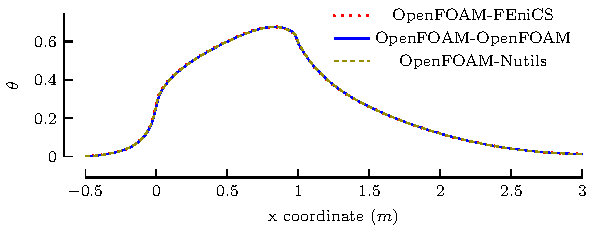
\includegraphics[width=0.9\textwidth]{figs/plate-result/plot_10s.pdf}
\end{center}
\caption{Flow over a heated plate CHT tutorial: Comparison of non-dimensional temperature values $\theta$ at time $t=10s$  along a line $0.01m$ above the bottom of the channel for different combinations of solvers. $x\in\left[-0.5,0\right]$ describes the region of the channel upstream of the plate, $x\in\left[0,1\right]$ the region where the channel and the plate are coupled and $x\in\left[1,3\right]$ the downstream region.}
\label{fig:cht_results}
\end{figure}

\subsection{Flow in a channel with an elastic perpendicular flap FSI tutorial} 

The most common use case of preCICE is FSI.
Often, one of the first case users aim to run is the Turek-Hron FSI3 benchmark~\cite{turek2006proposal}.
However, this case needs significant computational resources and specifications that are
not trivial to achieve with every solver out-of-the-box (e.g., parabolic inlet velocity profile in OpenFOAM).
A very common alternative is that of an elastic flap anchored at the bottom of a 2D channel flow as depicted in \autoref{fig:fsi_setup} and further described in the preCICE documentation\footnote{Documentation of this FSI tutorial: \url{https://precice.org/tutorials-perpendicular-flap.html}}.

\begin{figure}[h!]
\begin{center}
\begin{minipage}[t]{.55\textwidth}
\strut\vspace*{-\baselineskip}\newline
\input{figs/fsi/tikzcode.tex}
\end{minipage}
\hfill
\begin{minipage}[t]{.39\textwidth}
\begin{tabular}[t]{c S[table-format=6.2e2] s}
\multicolumn{3}{c}{Fluid: compressible Euler}\\
\midrule
$\text{Ma}_\infty$ & 1e-2 & \\  %https://github.com/DavidSCN/tutorials/blob/1fdfcf8aa22415868ef8fb8b3c5cf115f321eecf/perpendicular-flap/fluid-su2/euler_config_coupled.cfg#L44-L45
$p_\infty$ & 101325 & \pascal \\ %free-stream pressure (SU2 default), https://github.com/DavidSCN/tutorials/blob/1fdfcf8aa22415868ef8fb8b3c5cf115f321eecf/perpendicular-flap/fluid-su2/euler_config_coupled.cfg#L53-L54
$T_\infty$ & 288.15 & \kelvin  %https://github.com/DavidSCN/tutorials/blob/1fdfcf8aa22415868ef8fb8b3c5cf115f321eecf/perpendicular-flap/fluid-su2/euler_config_coupled.cfg#L56-L57
%\\
%$\alpha$ (AOA) & 0 & \degree (is the AOA relevant here?) %https://github.com/precice/tutorials/blob/5f4031fc7e45807dca787a525569b39a1909d2a3/FSI/flap_perp_2D/SU2-FEniCS/Fluid/euler_config_coupled.cfg#L39-L40
%\\ 
%$\rho_\infty$ & from $p_\infty$ and $T_\infty$ % We use TEMPERATURE_FS (https://github.com/su2code/SU2/blob/3cb709cfd29d6d75dfe53972b5aaa7a08294b9b5/config_template.cfg#L166) -> https://su2code.github.io/docs_v7/Physical-Definition/#thermodynamic-state
%\\
%$u_{\infty}$ & from $\text{Ma}_\infty$ and thermodynamics  %https://github.com/precice/tutorials/blob/master/FSI/flap_perp_2D/SU2-FEniCS/Fluid/euler_config_coupled.cfg#L91, https://github.com/precice/tutorials/blob/45f68c946f3d71536af4b0ed0fa5c0fa8168380a/FSI/flap_perp_2D/SU2-FEniCS/Fluid/euler_config_coupled.cfg#L91 -> https://su2code.github.io/docs_v7/Physical-Definition/#mach-number-and-velocity
\\[.5em]
\multicolumn{3}{c}{Fluid: incompressible Navier-Stokes}\\
\midrule
$u_{\infty}$ & 10 & \meter\per\second \\ %https://github.com/precice/tutorials/blob/5f4031fc7e45807dca787a525569b39a1909d2a3/FSI/flap_perp_2D/OpenFOAM-FEniCS/Fluid/0.orig/U#L13
$\nu_f$ & 1 & \meter\squared\per\second \\  %https://github.com/DavidSCN/tutorials/blob/af4cbce49567a593a621dda9173da8f694415456/perpendicular-flap/fluid-openfoam/constant/transportProperties#L13
$\rho_f$ & 1 & \kilogram\per\meter\cubed %https://github.com/precice/tutorials/blob/5f4031fc7e45807dca787a525569b39a1909d2a3/FSI/flap_perp_2D/OpenFOAM-FEniCS/Fluid/system/preciceDict#L53
%\\
%$\mu_f$ & $\frac{\nu_f}{\rho_f} = 1$  %https://en.wikipedia.org/wiki/Viscosity#Dynamic_and_kinematic_viscosity
\\[.5em]

\multicolumn{3}{c}{Solid}\\
\midrule
$E$& 4e6 & \newton\per\meter\squared \\  % FEniCS: https://github.com/precice/tutorials/blob/3ddf707ae306981aa1967bfb517eed235829f023/perpendicular-flap/solid-fenics/perp-flap.py#L30, CCX: https://github.com/precice/tutorials/blob/3ddf707ae306981aa1967bfb517eed235829f023/perpendicular-flap/solid-calculix/flap.inp#L6, deal.II: https://github.com/precice/tutorials/blob/3ddf707ae306981aa1967bfb517eed235829f023/perpendicular-flap/solid-dealii/linear_elasticity.prm#L26-L30
$\nu_s$ & 3e-1 & \\  % https://github.com/precice/tutorials/blob/5f4031fc7e45807dca787a525569b39a1909d2a3/FSI/flap_perp_2D/OpenFOAM-FEniCS/Solid/perp-flap.py#L31
$\rho_s$ & 3e3 & \kilogram\per\meter\cubed \\  % https://github.com/precice/tutorials/blob/5f4031fc7e45807dca787a525569b39a1909d2a3/FSI/flap_perp_2D/OpenFOAM-FEniCS/Solid/perp-flap.py#L29
\end{tabular}
\end{minipage}
\end{center}
\caption{Flow in a channel with an elastic perpendicular flap FSI tutorial: 
The setup is depicted on the left and physical parameters are listed in the table on the right. 
The bottom of the flap is clamped, the solid participant reads forces at the interface, while the fluid participant reads displacement values. The inflow velocity at the channel inlet is
$\SI{10}{\meter / \second}$ and the outflow sets a zero velocity gradient. $\text{Ma}_\infty$, $p_\infty$, $T_\infty$, $u_{\infty}$: Mach number, pressure, temperature, and velocity at the inflow. $\nu_f$, $\rho_f$: kinematic viscosity and density of the fluid.
$E$: Young's modulus. $\nu_s$: Poisson's ratio of the solid. $\rho_s$: density of the solid. $z$ is the out-of-plane thickness: even if the coupled case is described as 2D, OpenFOAM and CalculiX are still 3D solvers.}
\label{fig:fsi_setup}
\end{figure}

For the fluid participant, the user can choose between:
\begin{enumerate}
  \item the incompressible OpenFOAM solver pimpleFoam,
  \item an incompressible CFD solver written in Nutils, or
  \item the compressible CFD solver of SU2.
\end{enumerate}

For the solid participant, the user can choose among:
\begin{enumerate}
  \item the linear structure solver of CalculiX with linear, rectangular finite elements,
  \item a linear structure solver provided with the deal.II adapter, using fourth order, rectangular finite elements, or
  \item a linear structure solver example in FEniCS, using quadratic, triangular finite elements.
\end{enumerate}

All possible combinations ($\{\text{OpenFOAM, Nutils, SU2}\} \times \{\text{CalculiX, deal.II, FEniCS}\}$)
use the same preCICE configuration file and the user can select any combination. The fluid solvers read absolute displacement values at the interface (Dirichlet boundary condition) and write forces, while all solid solvers read forces (Neumann boundary condition) and write absolute displacements.
Some of the adapters also support additional coupling fields, for example relative displacement or stresses, but the employed combination here works with all involved adapters. By default, the tutorial is configured with RBF data mappings and a parallel-implicit coupling scheme using IQN-ILS acceleration.

A quantity that is commonly monitored in this scenario is the displacement of the tip of the flap. We track this quantity using a preCICE watchpoint and compare the results across different solver combinations in~\autoref{fig:fsi_results}. \autoref{fig:fsi_paraview} shows a direct comparison snapshot of an FSI simulation with an incompressible and a compressible fluid solver.



\begin{figure}[h!]
\begin{center}
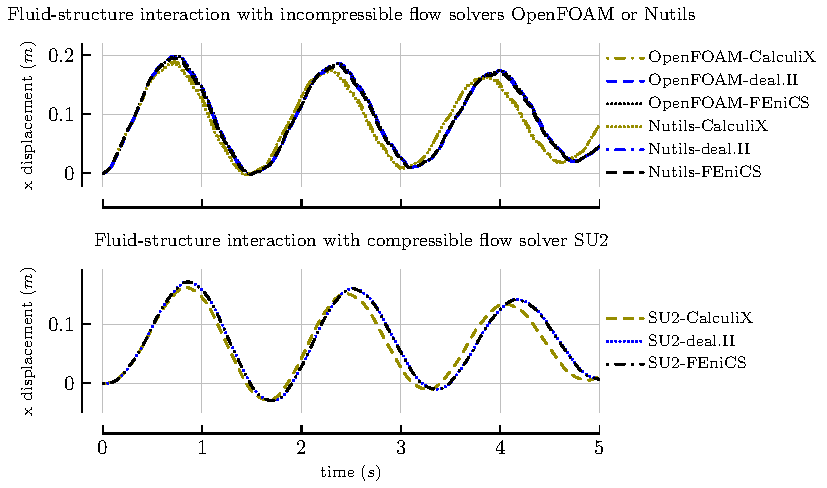
\includegraphics[scale=1]{figs/fsi-result/plot_small.pdf}
\end{center}
\caption{Flow in a channel with an elastic perpendicular flap FSI tutorial: Comparison of the flap tip displacement for different combinations of solvers. The upper plot shows the results for an incompressible flow computed with Nutils or OpenFOAM. The lower plot shows the results for compressible flow computed with SU2. Incompressible and compressible flow give qualitatively different results, as expected. Good agreement within each class of flow simulation is achieved when using FEniCS or deal.II as solid solver. Using CalculiX as solid solver leads to different results, presumably due to the use of linear elements. The CalculiX adapter is only capable of handling quasi 2D-3D cases with out-of-plane thickness for linear elements.}
\label{fig:fsi_results}
\end{figure}

\begin{figure}[h!]
\begin{center}
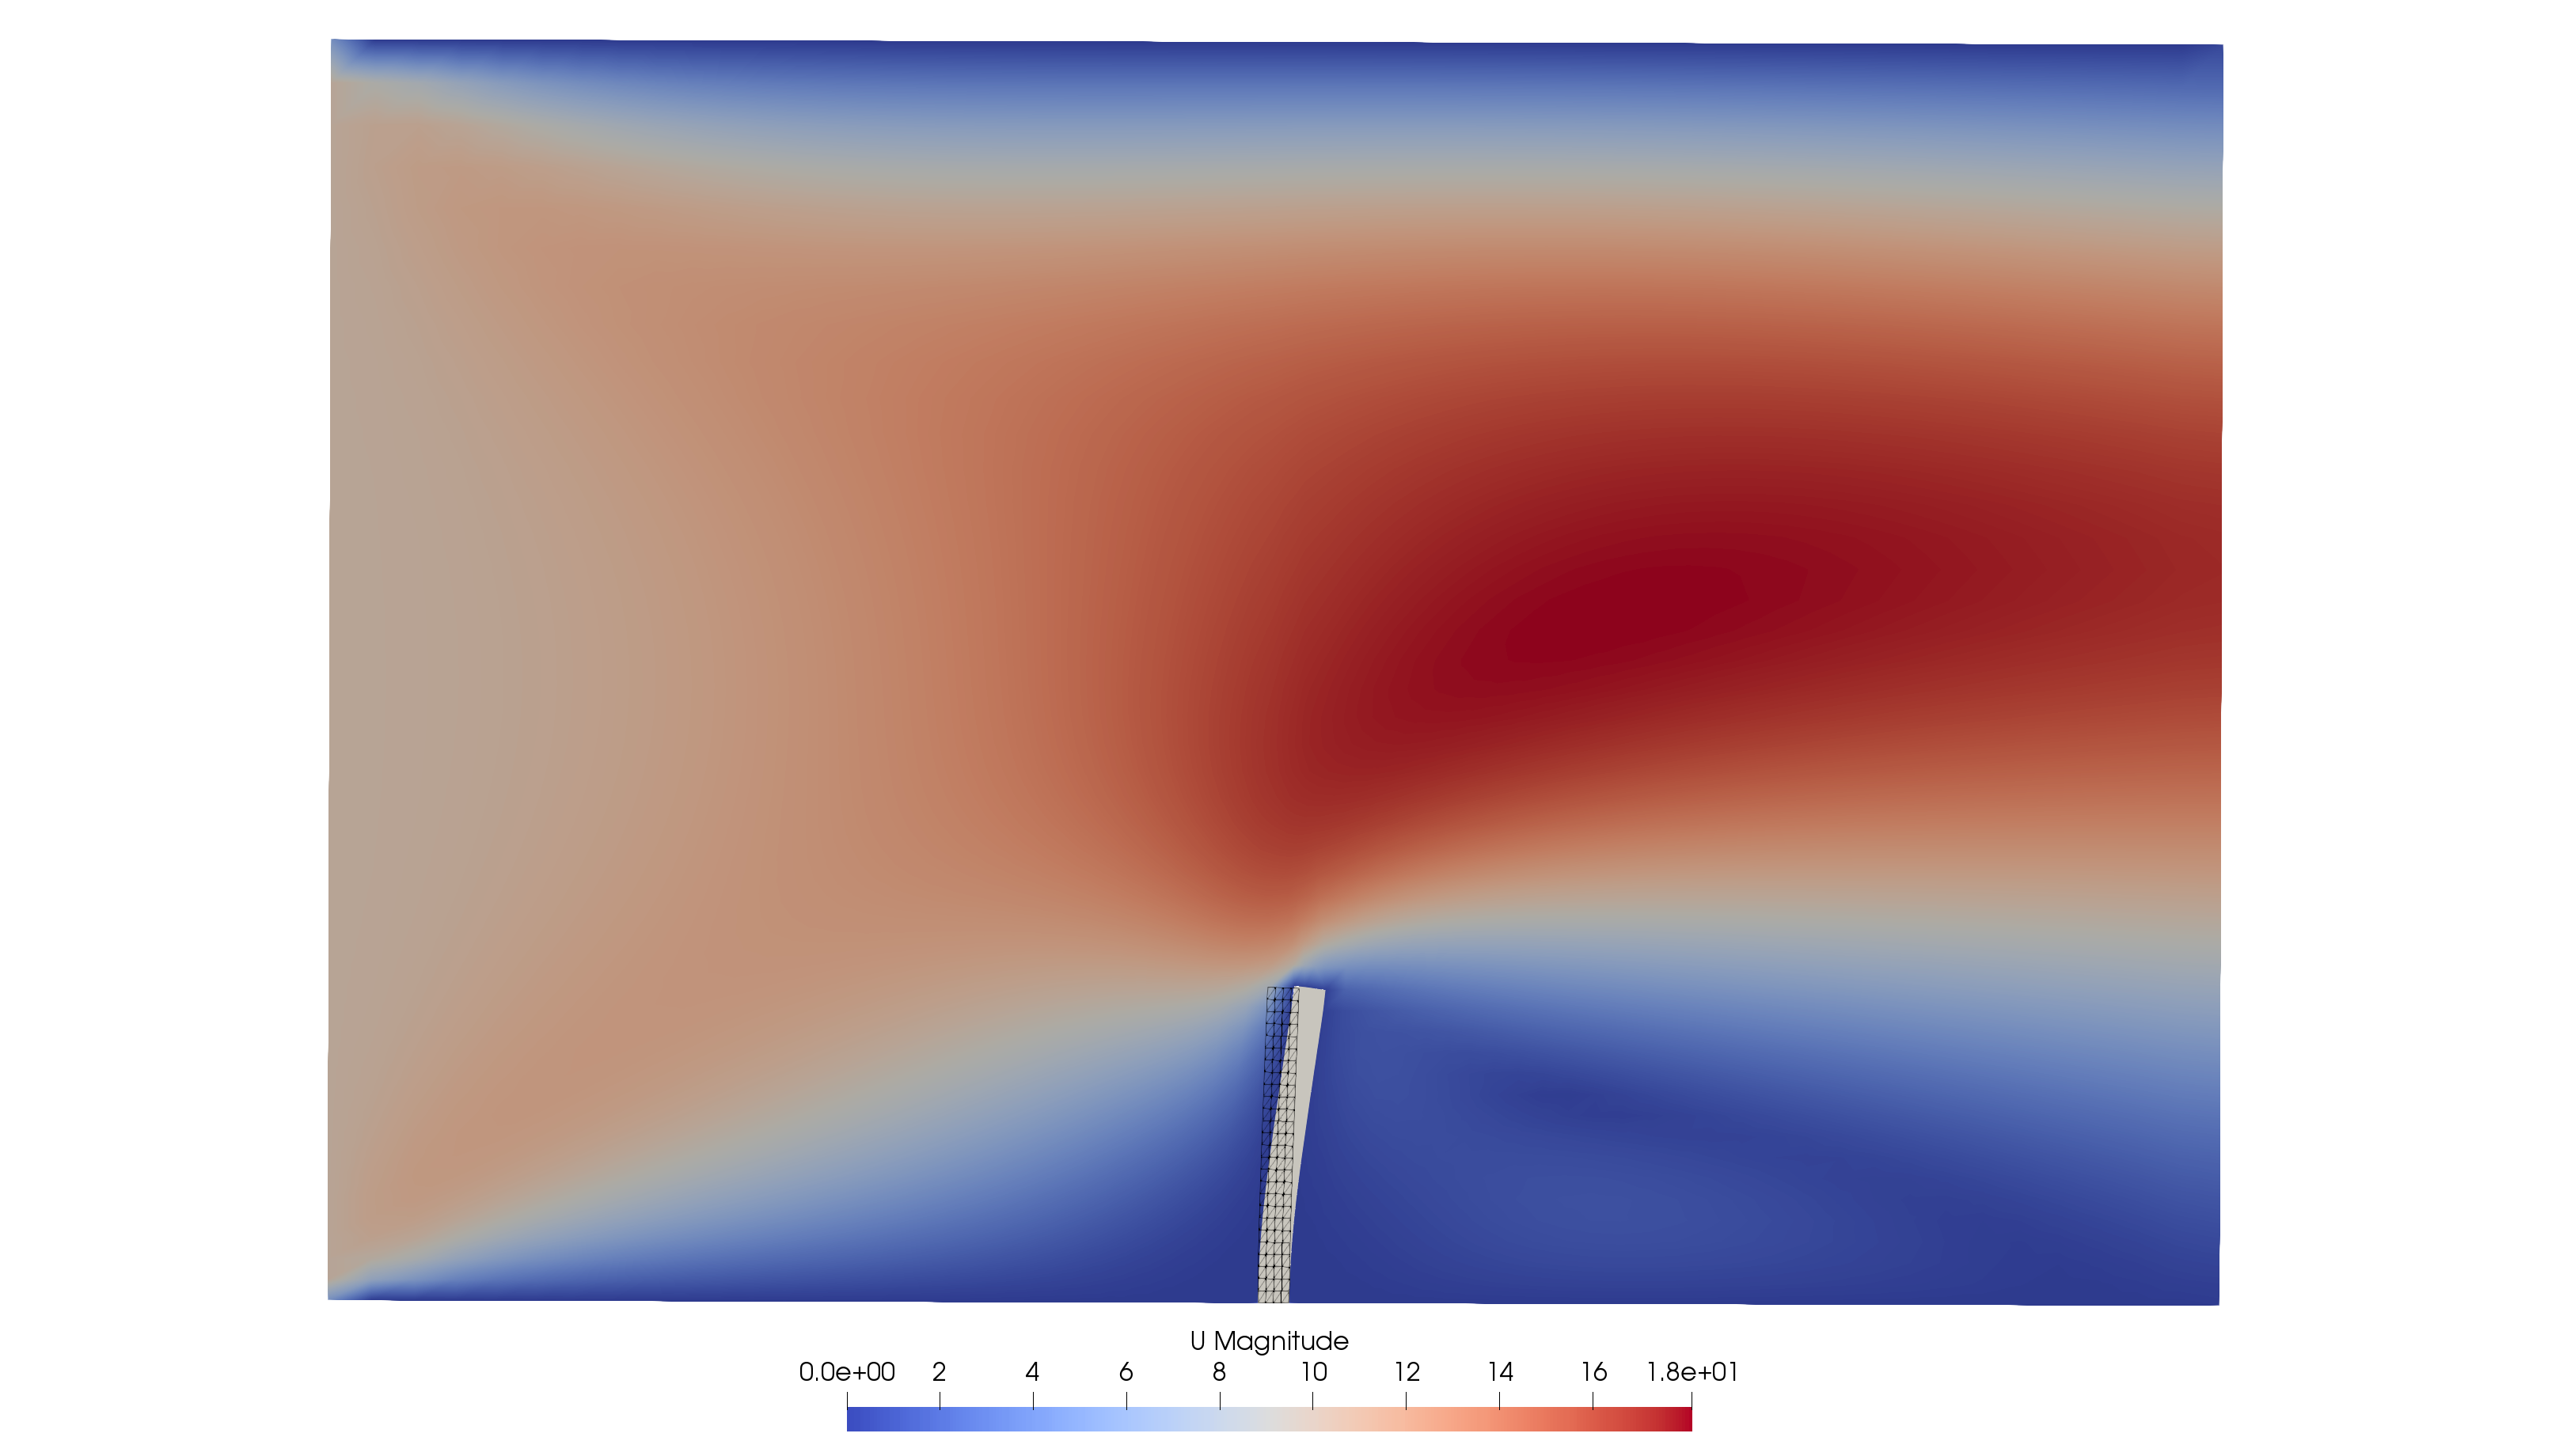
\includegraphics[width=\textwidth]{figs/fsi-paraview/FEniCS-OF-SU2-overlay.png}
\end{center}
\caption{Flow in a channel with an elastic perpendicular flap FSI tutorial: Visualization of flow field and deformed flap at time $t=2s$ using OpenFOAM as fluid and FEniCS as solid solver. For comparison, the deformed solid mesh of an SU2-FEniCS simulation is shown in black to make the difference between FSI with a compressible and an incompressible fluid simulation visible.}
\label{fig:fsi_paraview}
\end{figure}
